\chapter{Creación del Certificado Personal}

\section{Enunciado}

\textbf{5.1. Configuración de nuestra cuenta en Thunderbird para el empleo de OpenPGP}

Es parte del trabajo a realizar la búsqueda activa de información al respecto. En cualquier caso, se
pueden distinguir algunas etapas previas a la realización del envío del correo seguro:

\begin{itemize}[label=\textbullet]
    \item Antes de comenzar esta parte el estudiante podría eliminar de la configuración del
    Thunderbird toda la configuración realizada en el apartado anterior, eliminando el certificado
    S/MIME de la parte 2 \dots pero no lo aconsejamos, ya, el programa Thunderbird permite
    que coexistan configuraciones de S/MIME y OpenPGP, con el empleo habitual de
    mensajes sin cifrar ni firmar por ninguno de los dos sistemas. Es decir, si nuestro interlocutor
    no está almacenado en ninguna de las dos bases de datos de direcciones asociadas a clave
    pública SSL u OpenPGP, el comportamiento del Thunderbird será idéntico al convencional,
    y siempre se podrá configurar Thunderbird para que en su comportamiento por defecto, realice
    envíos cifrados, firmados (mediante OpenPGP y OpenSSL) o sin seguridad a direcciones
    asociadas a una clave pública o certificado X.509.
    \item A continuación, acceder en el menú superior a la opción Herramientas / Configuración de
    cuenta que abre una nueva pestaña, y en el menú de la izquierda seleccionar, abriendo la
    configuración de la cuenta escogida, la opción ``Generate OpenPGP Key''. En la pantalla
    siguiente, indicar que la clave no expira y el tipo de clave y tamaño recomendado. Finalizada
    la generación de las claves, se regresa a la pantalla anterior donde vemos que ya están
    activadas las claves OpenPGP para la cuenta seleccionada. Es importante asegurarnos de
    que NO hemos activado el cifrado por defecto ni el envío de firmas de manera
    predeterminada.
    \item A partir de ese momento, ya podríamos enviar mensajes firmados (todavía sin cifrar) con
    OpenPGP haciendo uso de la opción ``Seguridad'' de la pantalla de envío de mensajes y
    activando la casilla correspondiente, pero no tendría mucho sentido hacerlo a quién no tenga
    habilitada esta funcionalidad de correo seguro OpenPGP.
    \item Ahora, aconsejamos en esa misma pestaña, pulsar de nuevo el botón de ``OpenPGP Key
    Manager'' y seleccionando la clave recién creada, usar la opción de ``File/Backup secret keys
    to file'' para hacer una copia de la clave privada con contraseña, para conservarla en lugar
    seguro y acto seguido, la opción de ``File/Export Public Key to file''. Este último fichero
    puede ser enviado a cualquier compañero con el que queramos hacer una prueba de envío de
    mensaje firmado y cifrado, ya que sólo se puede cifrar un mensaje a una dirección de correo
    de la que tengamos su clave pública. Si enviamos el fichero de clave pública a un compañero,
    él podrá desde este mismo programa usar la opción inversa de ``File/Import Public Keys
    from File'' y validar nuestra clave pública. Es decir, una vez se hayan intercambiado las
    claves públicas entre dos o más compañeros, también se podrán intercambiar mensajes
    cifrados.
    \item Como alternativa más cómoda, se pueden intercambiar mensajes sólo firmados y los
    receptores de cada mensaje pueden incorporar la clave pública del remitente al almacén de
    claves de la herramienta ``OpenPGP Key Manager'' antes indicada, a continuación darle
    validez a la clave, y a partir de ese momento, se pueden enviar mensajes tanto firmados como
    cifrados.
\end{itemize}

Por tanto, repetimos que es muy conveniente, siempre que se pueda, practicar entre compañeros el
envío de mensajes firmados y cifrados. Si A le envía a B un mensaje firmado y su clave pública, B
dispondrá de la clave pública de A y podrá cifrar mensajes hacia él, sin necesidad de importar
manualmente la clave. Por tanto, esta parte del trabajo finaliza cuando podemos ver (y capturar) en
la pantalla de Thunderbird el mensaje cifrado y firmado por el compañero.

Es extremadamente importante que, una vez recibido el mensaje del compañero firmado y cifrado,
procedamos a importar su clave pública y a asignarle la máxima confianza a su clave. Hasta que
estos dos pasos no estén realizados, la pantalla que muestra el mensaje firmado y cifrado del
compañero no tendrá un ``sello verde'' en la etiqueta que indica que está firmado con una clave de
confianza. Este sello estará marcado en azul cuando aún no se ha importado la clave y en amarillo
hasta que no se confiera máxima confianza a la clave del compañero. No se aceptará una entrega
que no indique explícitamente el sello verde y capturas de las dos operaciones necesarias para que
este aparezca.

\section{Descripción teórica}

Un \textbf{certificado digital X.509} es un documento electrónico que vincula una identidad (nombre, correo electrónico, organización) con una clave pública. Esta vinculación está firmada por una \textbf{Autoridad de Certificación (CA)}, lo que permite a terceros confiar en que esa clave pública pertenece realmente a la identidad indicada.

El proceso de creación de un certificado personal implica los siguientes pasos:

\begin{enumerate}
    \item \textbf{Generar un par de claves} (pública y privada) para el usuario.
    \item \textbf{Crear una solicitud de firma (CSR)}: documento que contiene la clave pública y los datos del solicitante.
    \item \textbf{Firmar el CSR} con el certificado y clave de la CA raíz, generando el certificado final (.crt).
    \item \textbf{Empaquetar en PKCS\#12}: agrupar certificado y clave privada en un único fichero protegido (.p12) para su importación en aplicaciones.
\end{enumerate}

En esta práctica se utiliza un certificado raíz proporcionado por la asignatura (\texttt{certificadoRaiz.crt} y \texttt{certificadoRaiz.key}, protegido con la contraseña \texttt{SEGURIDAD}) como CA que firma nuestro certificado personal.

\section{Paso a) -- Descargar el certificado raíz}

Se descargan los ficheros \texttt{certificadoRaiz.crt} (parte pública) y \texttt{certificadoRaiz.key} (clave privada, protegida con contraseña \texttt{SEGURIDAD}) desde la página de la asignatura y se colocan en el directorio de trabajo.

\section{Paso b) -- Crear la clave del certificado personal}

Se genera una clave privada RSA protegida con cifrado AES-256:

\begin{lstlisting}[caption=Generación de la clave privada del certificado personal]
openssl genpkey -algorithm RSA -out certificadoPersonal.key -aes256
\end{lstlisting}

OpenSSL solicita una contraseña para proteger la clave privada. Esta contraseña será necesaria cada vez que se utilice la clave (por ejemplo, al firmar el CSR o al descifrar mensajes).

\begin{figure}[H]
    \centering
    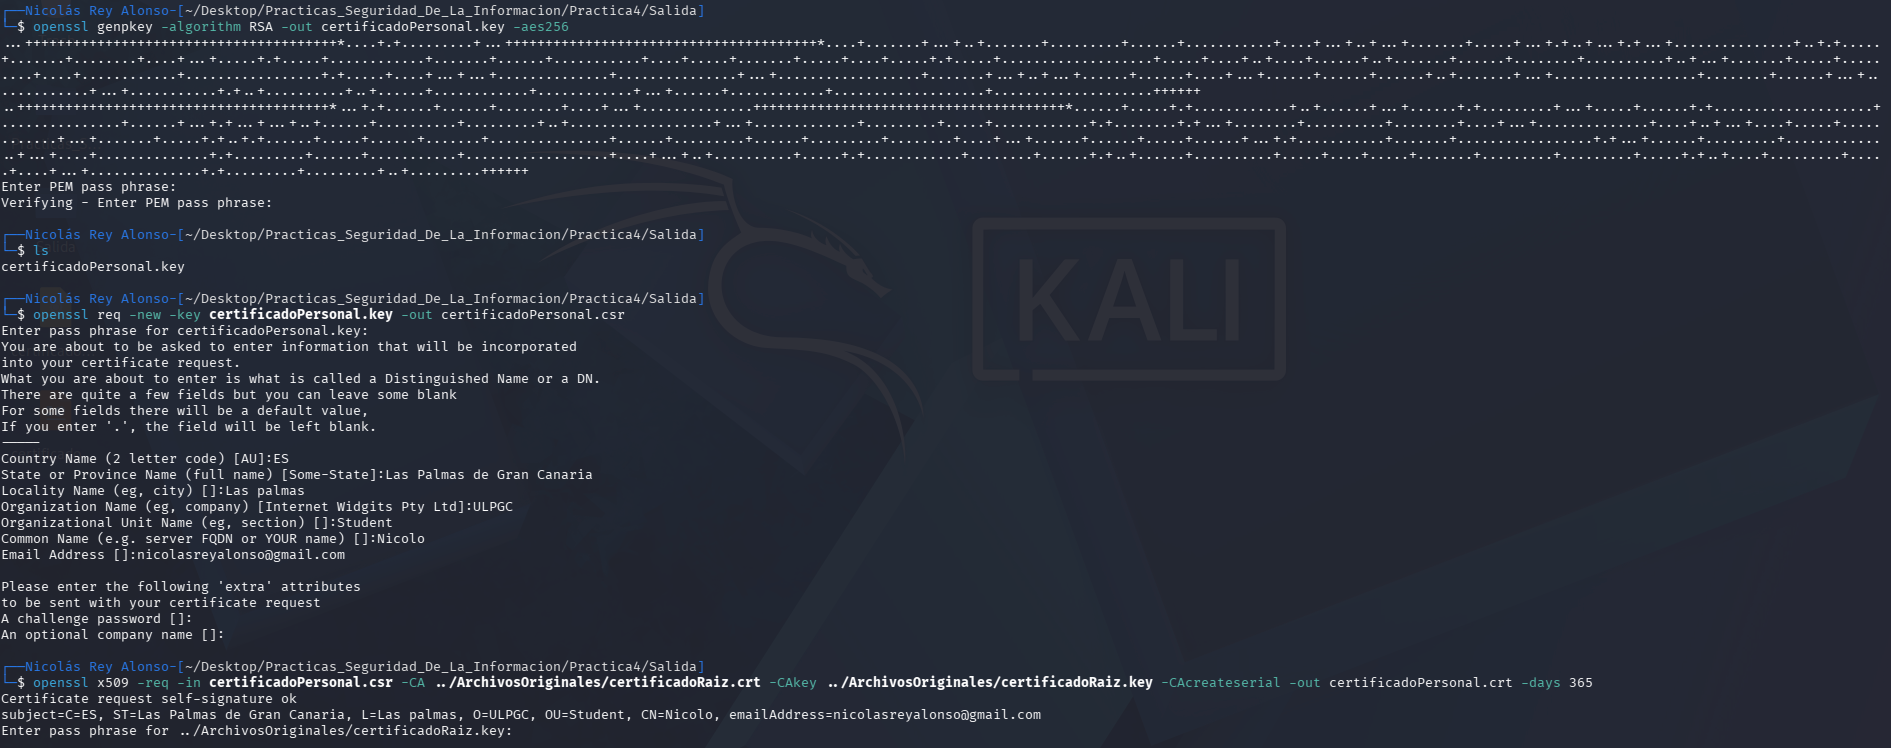
\includegraphics[width=\textwidth]{Imagenes/1.1.1.png}
    \caption{Generación de la clave personal y creación del CSR en terminal}
    \label{fig:creacion_clave_csr}
\end{figure}

\section{Paso c) -- Crear el CSR (Certificate Signing Request)}

El CSR incluye la clave pública y los datos identificativos del solicitante (país, organización, nombre, correo):

\begin{lstlisting}[caption=Creación del CSR]
openssl req -new -key certificadoPersonal.key -out certificadoPersonal.csr
\end{lstlisting}

Durante el proceso se introducen los campos del certificado:

\begin{itemize}[label=\textbullet]
    \item \textbf{C} (Country): ES
    \item \textbf{O} (Organization): ULPGC -- Seguridad de la Información
    \item \textbf{OU} (Organizational Unit): EII
    \item \textbf{CN} (Common Name): Nicolás Rey Alonso
    \item \textbf{Email}: dirección de correo personal
\end{itemize}

\section{Paso d) -- Firmar el CSR con el certificado raíz}

Se firma el CSR utilizando el certificado raíz y su clave privada, generando nuestro certificado personal con validez de 365 días:

\begin{lstlisting}[caption=Firma del CSR con el certificado raíz]
openssl x509 -req -in certificadoPersonal.csr \
    -CA certificadoRaiz.crt -CAkey certificadoRaiz.key \
    -CAcreateserial -out certificadoPersonal.crt -days 365
\end{lstlisting}

Se introduce la contraseña \texttt{SEGURIDAD} que protege \texttt{certificadoRaiz.key}. El resultado es el fichero \texttt{certificadoPersonal.crt} que contiene nuestra clave pública firmada por la CA raíz.

\begin{figure}[H]
    \centering
    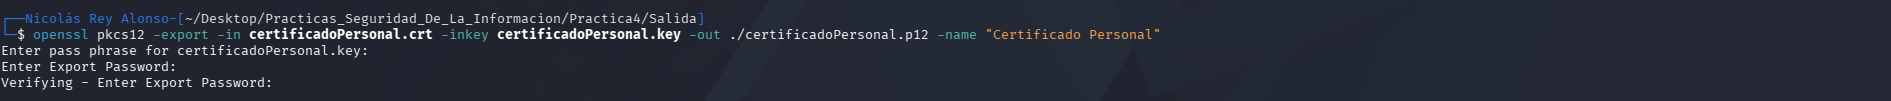
\includegraphics[width=\textwidth]{Imagenes/1.1.2.png}
    \caption{Firma del CSR y creación del fichero PKCS\#12}
    \label{fig:firma_csr_p12}
\end{figure}

\section{Paso e) -- Crear el fichero PKCS\#12}

El formato PKCS\#12 (.p12) empaqueta el certificado personal y la clave privada en un único fichero protegido con contraseña, adecuado para importar en clientes de correo como Thunderbird:

\begin{lstlisting}[caption=Creación del fichero PKCS\#12]
openssl pkcs12 -export -in certificadoPersonal.crt \
    -inkey certificadoPersonal.key \
    -out certificadoPersonal.p12 -name "Certificado Personal"
\end{lstlisting}

El comando solicita:
\begin{enumerate}
    \item La contraseña de \texttt{certificadoPersonal.key} (la que creamos en el paso b).
    \item Una nueva contraseña de exportación para proteger el fichero \texttt{.p12}.
\end{enumerate}

\section{Ficheros resultantes}

Tras completar el proceso, se dispone de los siguientes ficheros:

\begin{table}[H]
    \centering
    \caption{Ficheros generados en la creación del certificado}
    \begin{tabularx}{\textwidth}{l|l|X}
        \toprule
        \textbf{Fichero} & \textbf{Formato} & \textbf{Contenido} \\
        \midrule
        certificadoPersonal.key & PEM & Clave privada RSA cifrada con AES-256 \\
        certificadoPersonal.crt & PEM & Certificado personal (clave pública firmada por la CA) \\
        certificadoPersonal.p12 & PKCS\#12 & Clave privada + certificado en un solo fichero \\
        \bottomrule
    \end{tabularx}
\end{table}

El fichero \texttt{certificadoPersonal.csr} se elimina tras la firma, ya que no es necesario conservarlo.
